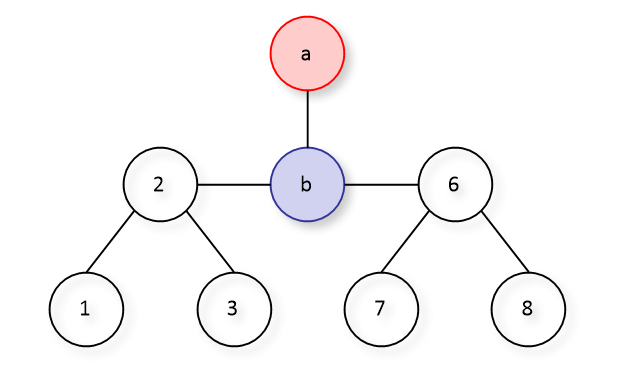
\includegraphics{sot-ex1pic.png}


다음 그림은 \bf{예제 입력 1}에서 주어진 \bf{트리}의 모습이다. 이 문제에서 '\bf{트리}'란 사이클이 없는 단순 연결 그래프를 의미하며, 여기서 '사이클'이란 어느 한 정점에서 출발해 같은 정점을 두 번 이상 방문하지 않고 시작점으로 돌아올 수 있는 경로를 말한다. 주어진 예제 그림은 '사이클이 없는 단순 연결 그래프'의 모습을 만족하고 있다.


이 예제의 경우 근성이 복제할 수 있는 정점 데이터의 최대 개수는 3개이다. 근성이 가능한 최적의 행동 중 하나는, \bf{기다리기}를 사용하지 않고 4(b)-2-1로 이동하며 매 정점마다 \bf{복제하기}를 사용하는 것이다.
